\documentclass[a4paper, 12pt]{article}

%%% Работа с русским языком
\usepackage{cmap}					% поиск в PDF
\usepackage{mathtext} 				% русские буквы в формулах
\usepackage[T2A]{fontenc}			% кодировка
\usepackage[utf8]{inputenc}			% кодировка исходного текста
\usepackage[russian]{babel}	% локализация и переносы

%%% Дополнительная работа с математикой
\usepackage{amsmath,amsfonts,amssymb,amsthm,mathtools} % AMS
\usepackage{icomma} % "Умная" запятая: $0,2$ --- число, $0, 2$ --- перечисление

%% Номера формул
%\mathtoolsset{showonlyrefs=true} % Показывать номера только у тех формул, на которые есть \eqref{} в тексте.

%% Шрифты
\usepackage{euscript}	 % Шрифт Евклид
\usepackage{mathrsfs} % Красивый матшрифт

%% Поля
\usepackage[left=2cm,right=2cm,top=2cm,bottom=2cm,bindingoffset=0cm]{geometry}

%% Русские списки
\usepackage{enumitem}
\makeatletter
\AddEnumerateCounter{\asbuk}{\russian@alph}{щ}
\makeatother

%%% Работа с картинками
\usepackage{graphicx}  % Для вставки рисунков
\graphicspath{{images/}{images2/}}  % папки с картинками
\setlength\fboxsep{3pt} % Отступ рамки \fbox{} от рисунка
\setlength\fboxrule{1pt} % Толщина линий рамки \fbox{}
\usepackage{wrapfig} % Обтекание рисунков и таблиц текстом

%%% Работа с таблицами
\usepackage{array,tabularx,tabulary,booktabs} % Дополнительная работа с таблицами
\usepackage{longtable}  % Длинные таблицы
\usepackage{multirow} % Слияние строк в таблице

%% Красная строка
\setlength{\parindent}{2em}

%% Интервалы
\linespread{1}
\usepackage{multirow}

%% TikZ
\usepackage{tikz}
\usetikzlibrary{graphs,graphs.standard}

%% Верхний колонтитул
\usepackage{fancyhdr}
\pagestyle{fancy}

%% Перенос знаков в формулах (по Львовскому)
\newcommand*{\hm}[1]{#1\nobreak\discretionary{}
	{\hbox{$\mathsurround=0pt #1$}}{}}

%% Мои дополнения
\usepackage{float} %Добавляет возможность работы с командой [H] которая улучшает расположение на странице
\usepackage{gensymb} %Красивые градусы
\usepackage{graphicx}               % Импорт изображений
\usepackage{caption} % Пакет для подписей к рисункам, в частности, для работы caption*
\usepackage{indentfirst}


\begin{document}

\newcommand{\HRule}{\rule{\linewidth}{0.7mm}} % Defines a new command for the horizontal lines, change thickness here
	
	\begin{center}
		\large\textbf{Московский Физико-Технический Институт}\\ % Name of your university/college
		\large\textbf{(государственный университет)}
	
		\vfill
		
		\Large Лабораторная работа по курсу общей физики № 4.5.3\\[0.5cm] % Preambule of your document title
		
		
		\HRule
		\\[0.4cm]
		{ \huge \bfseries Сканирующий интерферометр}% Title of your document
		\\[0.4cm] 
		\HRule
		\\[0.5cm]
		
		\ \\
	\textbf{\large Автор:} \\	
	\large Лепарский Роман Б01-003\\ % Your name and something more, your group num for example
		\vfill
		\hspace*{-0.8 cm}
\includegraphics[width=100 pt]{frkt_logo}\\ % logo of your  company/university/college
		\large Долгопрудный, 2022 % location and year
	\end{center}

\newpage
\setcounter{page}{2}
\fancyfoot[c]{\thepage}
\fancyhead[L] {Работа № 4.5.3} % some information in page header
\fancyhead[R]{}

\section{Аннотация}

\textbf{Цель работы:} ознакомление с интерференцией на двух щелях,
устройством и принципом действия интерферометра Релея и с его
применением для измерения показателей преломления газов.

\textbf{Приборы и материалы:} технический интерферометр ИТР-1, светофильтр, баллон с углекислым газом, сильфон, манометр, краны.

\section{Теоретические сведения}

\subsection{Зависимость показателя преломления газа от давления}
Воспользуемся известной формулой диэлектрической проницаемости $\varepsilon$ для газа невзаимодействующих диполей:
\begin{equation*}
	\varepsilon = n^2 = 1 + 4\pi N\alpha
\end{equation*}
Тогда для связи разности показателей преломления $\delta n$ и давлений $\delta P$ имеем
\begin{equation*}
	\delta n = \frac{\alpha}{2k_BT}\delta P
\end{equation*} 
	
\section{Экспериментальная установка}
\begin{figure}[H]
	\centering
	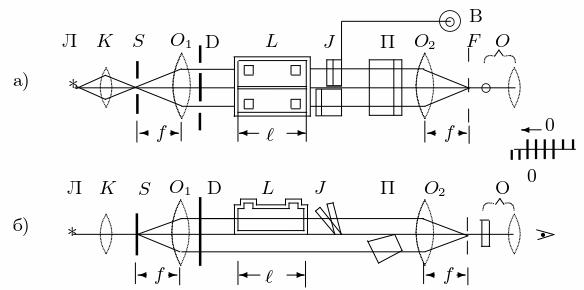
\includegraphics[scale = 0.7]{stand.jpg}
	\caption{Интерферометр Релея}
\end{figure}

Свет от источника, прошедший через тонкую щель $S$, разделяется на 2 когерентных луча. Нижняя их часть беспрепятственно проходит до линзы $O_2$ и образует в её фокальной плоскости неподвижную интерференционную картину. Верхняя же часть проходит через кювету, содержимое которой имеет другой показатель преломления, а затем через компенсатор Жамена, что позволяет подстроить интерференционную картину.

При малых дифракционных углах расстояние между соседними максимумами $\delta y$ зависит от длины волны $\lambda$, фокусного расстояния линзы $O_2$ - $f$ и расстояния между щелями $d$ следующим образом:
\begin{equation*}
 \delta y = f\frac{\lambda}{d}
\end{equation*} 
 При заполнении кюветы газом, с отличным от воздуха при атмосферном давлении показателем преломления, возникает дополнительная разность хода. Смещение верхней интерференционной картины относительно нижней на одну полосу означает изменение разности хода на $\lambda$. Таким образом
 \begin{equation*}
 	\delta n = m\frac{\lambda}{L}
 \end{equation*}
Или в более общем виде
\begin{equation*}
	n = n_\text{возд} + \frac{\Delta}{L}
\end{equation*}

\section{Обработка результатов}

\subsection{Калибровка компенсатора Жамена}
	Запишем в таблицу данные установки:
	\begin{table}[H]
		\centering
		\begin{tabular}{|l|l|l|l|}
			\hline
			$T$, K & $P$, кПа & $l$, см & $\lambda$, нм \\ \hline
			295    & 99,3     & 25      & $670 \pm 50$  \\ \hline
		\end{tabular}
	\end{table}

Данные для построения калибровочного графика:
\begin{table}[H]
	\centering
	\begin{tabular}{|l|l|}
		\hline
		$m$, ед & $\Delta$, дел \\ \hline
		-7      & 0,05          \\ \hline
		-6      & 0,41          \\ \hline
		-5      & 0,76          \\ \hline
		-4      & 1,09          \\ \hline
		-3      & 1,45          \\ \hline
		-2      & 1,84          \\ \hline
		-1      & 2,16          \\ \hline
		0       & 2,5           \\ \hline
		1       & 2,86          \\ \hline
		2       & 3,21          \\ \hline
		3       & 3,56          \\ \hline
		4       & 3,92          \\ \hline
		5       & 4,27          \\ \hline
		6       & 4,6           \\ \hline
		7       & 4,95          \\ \hline
	\end{tabular}
\end{table}

Построим калибровочный график
\begin{figure}[H]
	\centering
	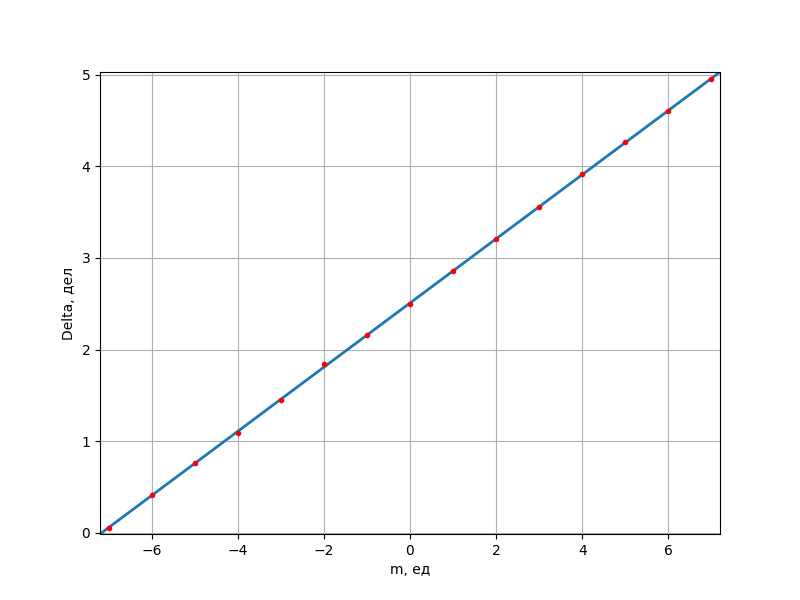
\includegraphics[scale = 0.7]{kalib.png}
	\caption{Калибровочный график}
\end{figure}

Обратный коэффициент наклона $k = 2.855 \pm 0,004$ $\lambda$/дел.

\subsection{Зависимость показателя преломления от давления воздуха}

Найдем зависимость показателя преломления $\delta n$ от разности давлений $\delta P$. Запишем результаты измерений в таблицу

\begin{table}[H]
	\centering
	\begin{tabular}{|l|l|l|l|}
		\hline
		$\delta P$, mmH2O & $\delta P$, Па & $\Delta$, дел & $\delta n \cdot 10^{-6}$ \\ \hline
		-1000             & -9800          & 6,22          & 28,46                    \\ \hline
		-900              & -8800          & 5,74          & 24,79                    \\ \hline
		-800              & -7800          & 5,35          & 21,80                    \\ \hline
		-700              & -6800          & 5,03          & 19,35                    \\ \hline
		-600              & -5800          & 4,66          & 16,52                    \\ \hline
		-500              & -4900          & 4,28          & 13,61                    \\ \hline
		-400              & -3900          & 3,91          & 10,78                    \\ \hline
		-300              & -2900          & 3,57          & 8,18                     \\ \hline
		-200              & -1900          & 3,17          & 5,12                     \\ \hline
		-100              & -900           & 2,83          & 2,52                     \\ \hline
		0                 & 0              & 2,5           & 0                        \\ \hline
		100               & 900            & 1,83          & -5,12                    \\ \hline
		200               & 1900           & 1,5           & -7,65                    \\ \hline
		300               & 2900           & 1,19          & -10,02                   \\ \hline
		400               & 3900           & 0,87          & -12,47                   \\ \hline
		500               & 4900           & 0,6           & -14,53                   \\ \hline
		600               & 5800           & 0,19          & -17,67                   \\ \hline
		700               & 6800           & -0,23         & -20,88                   \\ \hline
	\end{tabular}
\end{table}

Отложим измерения на графике

\begin{figure}[H]
	\centering
	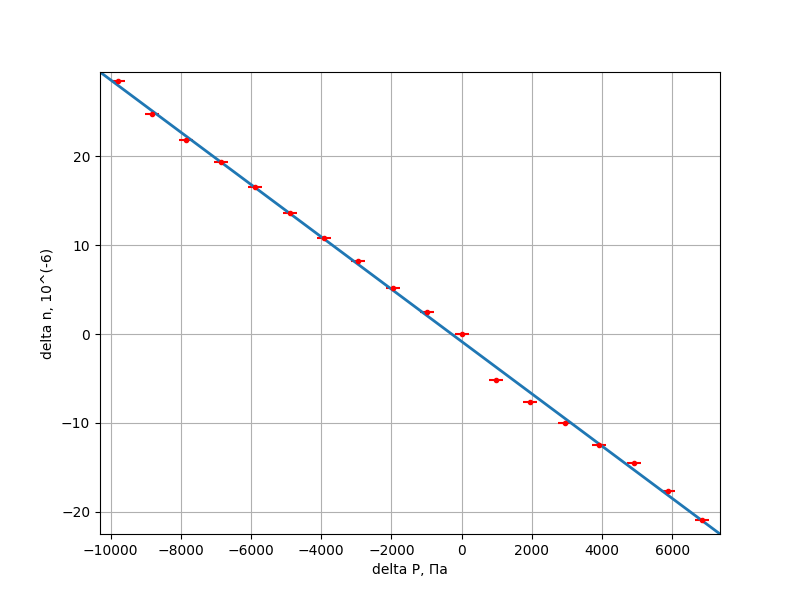
\includegraphics[scale = 0.7]{n_P.png}
	\caption{Зависимость $\delta n (\delta P)$}
\end{figure}

Коэффициент наклона $b = (-239 \pm 2) \cdot 10^{-11}$ 1/Па. Откуда средняя поляризуемость $\alpha = (1,946 \pm 0,016) \cdot 10^{-30}$. Табличное значение $\alpha = 1,7 \cdot 10^{-30}$.

Отсюда показатель преломления в условиях эксперимента
$$n = 1,00002372 \pm 0,00000019$$
И в нормальных условиях
\[
	n_0 = 1,0000260 \pm 0,0000002
\]
Табличное значение $n_0 = 1,0002926$

\subsection{Зависимость показателя преломления от концентрации CO2}

Запишем в таблицу отклонение компенсатора Жамена в зависимости от времени. И пересчитаем его в разность показателей преломления.
\begin{table}[H]
	\centering
	\begin{tabular}{|l|l|l|}
		\hline
		$t$, м & $\Delta$, дел & $\ln{\Delta}$ \\ \hline
		0      & 20,68         & 3,0291        \\ \hline
		1      & 19,47         & 2,9688        \\ \hline
		2      & 18,52         & 2,9188        \\ \hline
		3      & 17,48         & 2,8610        \\ \hline
		4      & 16,84         & 2,8237        \\ \hline
		5      & 16,02         & 2,7738        \\ \hline
		6      & 15,32         & 2,7291        \\ \hline
		7      & 14,17         & 2,6511        \\ \hline
		8      & 13,93         & 2,6340        \\ \hline
		9      & 13,30         & 2,5877        \\ \hline
		10     & 12,73         & 2,5439        \\ \hline
		11     & 12,25         & 2,5055        \\ \hline
		12     & 11,71         & 2,4604        \\ \hline
		13     & 11,22         & 2,4176        \\ \hline
		14     & 10,85         & 2,3841        \\ \hline
		15     & 10,44         & 2,3456        \\ \hline
		16     & 10,08         & 2,3105        \\ \hline
		17     & 9,72          & 2,2741        \\ \hline
		18     & 9,35          & 2,2353        \\ \hline
		19     & 9,03          & 2,2005        \\ \hline
		20     & 8,70          & 2,1633        \\ \hline
	\end{tabular}
\end{table}

Построим график данной зависимости в логарифмическом масштабе.
\begin{figure}[H]
	\centering
	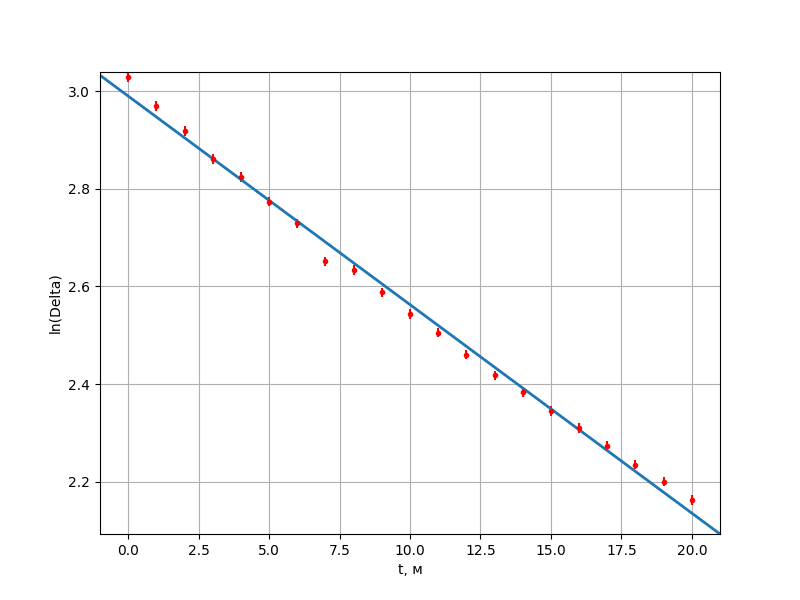
\includegraphics[scale = 0.7]{co2.png}
\end{figure}

Поскольку график практически линейный, можно говорить об экспоненциальном характере зависимости.

Пользуясь нулевым измерением, найдем коэффициент преломления углекислого газа. $n_{CO2} = n + \dfrac{\Delta}{L} = 1,0001836 \pm 0,0000004$. И при пересчете к нормальным условиям
\[
	n_{CO2_0} = 1,0002017 \pm 0,0000005
\]
Табличное значение данной величины: $1,000450$

\section{Вывод}

В данной работе мы ознакомились с устройством и принципом действия интерферометра Релея. А так же нашли коэффициенты преломления воздуха и углекислого газа в условиях эксперимента и в нормальных условиях.

\end{document}